
\documentclass[11pt]{article}
\usepackage{amssymb}
\usepackage{graphicx}
\usepackage{amsthm}
\usepackage{enumitem}
\usepackage{nameref}
\usepackage{indentfirst}
\setlength{\textheight}{9in} \setlength{\headheight}{.2in}
\setlength{\headsep}{0in} \setlength{\topmargin}{0in}


\newtheorem{thm}{Theorem}[section]
\newtheorem{lemma}[thm]{Lemma}
\newtheorem{definition}[thm]{Definition}

\let\olddefinition\definition
\renewcommand{\definition}{\olddefinition\normalfont}

\let\olddefinition\thm
\renewcommand{\thm}{\olddefinition\normalfont}


\begin{document}
\title{Graph Masking: Maintaining Neighborhoods in Graph Randomization}
\author{
	   Benjamin Caulfield \qquad Wesley Miller \qquad Malik Magdon-Ismail\\
        Rensselaer Polytechnic Institute\\
        Computer Science Department\\
        Troy, NY 12180\\
}



\maketitle

%Abstract

\noindent {\bf Abstract}\\
\indent Given a graph $G(V,E)$ and a natural number $k$, we define the $k-Neighborhood$  graph of G to be $G_k(V, E_k)$, where the edge $(u,v)$ is in $E_k$ if and only if there is a path $(u,v)$ of length less than or equal to $k$ in $G$. We would like to find a $masking$ of $G$, $G'$, such that $G$ and $G'$ share a $K-neighborhood$, but no edges in $G$ can be determined by studying $G'$ ($G'$ is sufficiently random). This paper provides two heuristic algorithms to solve this problem. The first modifies $G$ to get a new graph which is guaranteed to share a $k-Neighborhood$ with $G$, but may not be sufficiently random. The second algorithm builds the new graph by continuously adding edges to an originally empty graph. The new graph is sufficiently random from the original graph, but may not share the same $k-Neighborhood$.
\\\\


%Introduction
\section{Introduction}


\subsection{Motivation} 


\indent Social networks provide means to create and maintain meaningful connections between people. They foster environments where people can not only connect with people with whom they have a previous relationship, but with entirely new people as well. Without a proper way to introduce people to others with whom they may have relevant connections, there is little room for social networks to grow and provide anything worthwile to their users. \\

\indent As social networks, such as LinkedIn, hold all the data on connections between their users, they too hold the tools to make suggestions to users on which people to seek out for connections; however, this information must be used carefully. Users put their trust in the social networks that their private information will be kept safe and not disclosed to anyone else, so security is a major factor to be considered while trying to implement methods to expand the network.  \\

\indent In order to give the users relevant suggestions to expand their personal connections, a construction or product of a subset of the information held by the networks must be given such that it both is helpful to the users and does not infringe on the  privacy of others. \\

\subsection{Goal}

\indent The ultimate goal of this research is to find a k value such that the network can provide a given user with a list of his/her k-neighbors that satisfy the aforementioned conditions. The list of k-neighbors given must not reveal too much to users to prevent network adversaries from being able to reconstruct the graph to any reasonable extent but must be useful enough to provide helpful information to the users who make appropriate use of the network. \\

\subsection{Approach}

\indent This paper describes a method that looks at the connections between users to determine useful information to make available to a given user so that he/she may gain new meaningful connections. This includes a label-swapping algorithm and an edge adding algorithm. Algorithms were also designed to try to test the difficulty of accurately extracting any private information from the information given. All algorithms were evaluated for computational efficiency and data was taken to evaluate them overall.  \\

%Basic Definitions
\begin{dfn}
A \emph{graph} is a 2-tuple $G = (V,E)$, where $V = \{v_1,v_2,...,v_n\}$ is a set of vertices (nodes) and the set of edges is $E = \{e_1,e_2,...,e_m\} \subseteq V \times V$. All edges in $E$ are undirected. Unless otherwise stated, when discussing a graph $G=(V,E)$, $u,v,w \in V$ and $e \in E$. \\
\end{dfn}

\begin{dfn}
 A \emph{path} $P$ of length $l$ in $G$ is a sequence of edges in $E$ of the form $e_1', e_2', ...,e_l'$ such that $e_i' = (v,u)$ and $e_{i+1}' = (u,w)$ for all $i \in [1,l-1]$. If $e_1' = (v_0', v_1')$ and $e_l' = (v_{l-1}', v_l')$, then $P$ is a path from $v_0'$ to $v_l'$. \\
\end{dfn}

\begin{dfn}
Let $k$ be a positive integer. The \emph{k-neighborhood} of a node $v \in V$ in a graph $G = (V,E)$, denoted $N_k(v)$ is the set of all $u \in V$ where there exists a path from $v$ to $u$ of length less than or equal to $k$. The k-neighborhood of $G$ is the graph $N_k(G) = (V, E')$ where $(u,v) \in E'$ iff $v \in N_k(u)$. If $N_k(G) = G'$, we say that $G$ \emph{satisfies} $G'$. \\
\end{dfn}

\begin{dfn}
A \emph{masking} of a graph $G$ is a graph $G'$ which satisfies $N_k(G) = N_k(G')$. \\
\end{dfn}

\begin{dfn}
For an integer $k$ and graph $G$, we define the \emph{adjacency group} of a node $v \in V$ as the set of all $u \in V$ such that $N_k(v) = N_k(u)$. We can see that adjacency groups are equivalence classes. \\
\end{dfn}


%Label-Swapping
\section{Label-Swapping Algorithm}
\indent In this section, we present the \emph{label-swapping} algorithm which takes a graph $G$ and yields $G'$, a masking of $G$.This algorithm, as shown in figure \ref{fig:label-swap}, works by altering the original graph while maintaining the same $k-Neighborhood$. This is accomplished by partitioning the vertices of the graph into $adjacency$-$groups$.

\begin{figure}[htb]
	\begin{algorithmic}
		\renewcommand{\algorithmicrequire}{\textbf{Input:}}
		\renewcommand{\algorithmicensure}{\textbf{Output:}}
		\Require {List of Adjacency Groups $A$}
		\Ensure {Sorted List of Adjacency Groups $A'$}
		\State {Declare kTree $T$}
		\ForAll {$a \in A$}
			\State {Insert $a$ into a branch of $T$ sorting criteria}
		\EndFor
		\State {Extract sorted list of adjacency groups from $T$ as $A'$}
		\State \Return {$A'$}
	\end{algorithmic}
	\caption{Pseudocode for the kSort Algorithm.}
	\label{fig:kSort}
\end{figure}

\begin{figure}[htb]
	\begin{algorithmic}
		\renewcommand{\algorithmicrequire}{\textbf{Input:}}
		\renewcommand{\algorithmicensure}{\textbf{Output:}}
		\Require {Graph $G = (V, E)$, Integer $k$}
		\Ensure {Graph $G' = (V, E')$}
		\ForAll {$v \in V$}
			\State {calculate $N_k(v)$}
		\EndFor
		\State {Apply ksort algorithm to find adjacency groups}
		\ForAll {$A \in Adjacency Groups$}
			\State {find a valid swapping on $A$}
		\EndFor
		\ForAll {$(u,v) \in E$}
			\State {add edge $(Swap(u),Swap(v))$ to $E'$}
		\EndFor
		\State \Return {$G' = (V,E')$}
	\end{algorithmic}
	\caption{Pseudocode for the label-swapping algorithm.}
	\label{fig:label-swap}
\end{figure}

\indent The label-swapping algorithm, as shown in figure \ref{fig:label-swap} works by finding all maximal adjacency-groups and applying a random swapping to each one. The new graph formed by applying these swappings must have the same k-Neighborhood as the original graph (see Theorem 3.1); however, it may be possible to determine edges in the original graph from the new graph.
\\

\begin{figure}[ht]
  \centering
  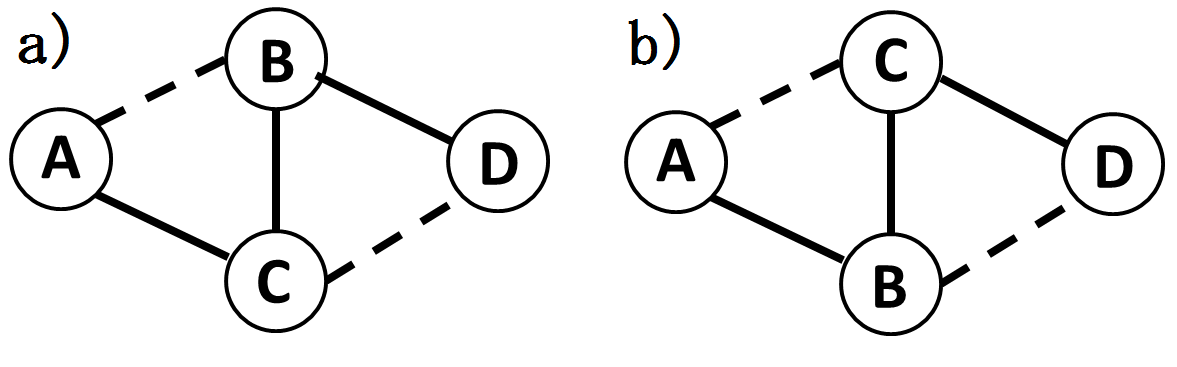
\includegraphics[scale=0.3 ]{Sample-Graph.png}
  \caption{In the above graphs, solid lines represent edges in the original graph and dotted lines represent edges that are only in the 2-Neighborhood graph (Note that all edges in the original graph are necessarily in the 2-Neighborhood graph). a)  The vertices B and C are in the same adjacency-group, while A and D are each in adjacency-groups of size 1. b) The result of applying a swapping to the adjacency group containing B and C, with the 2-Neighborhood graph remaining the same as the graph in (a).}
  \label{fig:sample graph}
\end{figure}


\begin{figure}[ht]
  \centering
  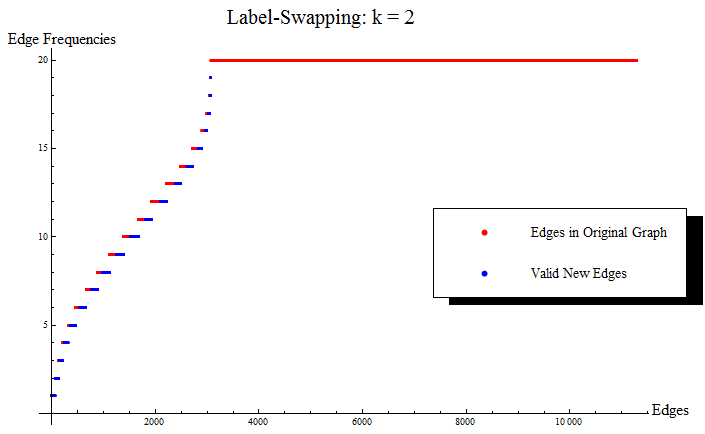
\includegraphics[scale=0.8 ]{s40_k_2_nomerge.png}
  \caption{The results from the label-swapping algorithm when run 20 times on the blog data when k=2.}
  \label{fig:s40-k=2-label-swap}
\end{figure}



\begin{thm}  \emph{Applying a swapping to a graph, G, will yield a graph, G', with the same k-Neighborhood graph as G.}
\end{thm}
\begin{proof}
\noindent Let $G_k'$ be the k-Neighborhood graph of $G'$ and $G_k$ be the k-Neighborhood graph of $G$. Assume $G_k'$ is not equal to $G_k$. Then (i) $G_k'$ contains an edge not in $G_k$ or (ii) $G_k$ contains an edge not in $G_k'$.  \\
\indent i) Let $(u,v)$ be an edge in $G_k'$ that's not in $G_k$. Since $G'$ was formed by $swappings$ on $G$, $u$ must have some label $x$ and $v$ must have some label $y$ in $G$, where $x$ and $y$ were in the adjacency-groups of $u$ and $v$, respectively, and $(x,y)$ is in $G_k$. But, since $u$ and $x$ are in the same adjacency-group, and $(x,y)$ is in $G_k$, then $(u,y)$ must be in $G_k$. Since $y$ and $v$ are in the same adjacecy-group and $(u,y)$ is in $G_k$, then $(u,v)$ is in $G_k$, and our assumption that $G_k'$ has an edge that is not in $G_k$ must be false.\\
\indent 			ii) Let $(u,v)$ be an edge in $G_k$ that is not in $G_k'.$ Let the nodes labeled $x$ and $y$ in $G$ be given the labels $u$ and $v$, respectively, in $G'$. Therefore, $u$ and $x$ share an adjacency-group, as do $v$ and $y$.  Since $(u,v)$ is in $G_k$ and $u$ and $x$ share an adjacency-group, then $(x,v)$ is in $G_k$. Likewise, since $v$ and $y$ share an adjacency-group and $(x,v)$ is in $G_k$, then $(x,y)$ is in $G_k$. This implies that $(u,v)$ must be in $G_k'$. Therefore, our assumption that $G_k$ has an edge that is not in $G_k'$ is false. \\
\indent Because (i) and (ii) are false, we can conclude that $G_k$ equals $G_k'$.\\
\end{proof}


%Merging Heuristics
\section{Merging Heuristics}
\indent Unfortunately, although the label-swapping algorithm yields perfectly satisfying graphs, it often doesn't sufficiently disguise a given graph.  In this section, we present a heuristic, called \emph{adjacency group merges} or simply \emph{merges}, that further randomizes a given graph but is not guaranteed to maintain the same k-neighborhood. 

\begin{dfn}
\noindent A \emph{merge} or \emph{merging} of a graph's adjacency groups combines similar adjacency groups into larger groups containing the union of their nodes based on their \emph{difference}. It runs deterministically and maps every pair of nodes to  the differencence value between their adjacency groups and merges adjacency groups of the first n that have not been involved in a previous merge. \\
\end{dfn}

\begin{dfn}
The \emph{difference} between adjacency groups $A$ and $B$ is the size of the symmetric difference of $N_k(v)$ and $N_k(u)$, for $v \in A$ and $u \in B$. 
\end{dfn}

\begin{figure}[htb]
	\begin{algorithmic}
		\tiny
		\renewcommand{\algorithmicrequire}{\textbf{Input:}}
		\renewcommand{\algorithmicensure}{\textbf{Output:}}
		\Require {graph $G=(V,E)$, k-neighborhoods $K= \{k_{1}, k_{2}, ...\}$, adjecency groups $A=\{a_{1}, a_{2}, ...\}$, limit L}
		\Ensure {adjecency groups $A'$}
		\ForAll {$v \in V$}
			\ForAll {$w \in W$ where $v \neq w$}
				\State {find $Diff(A(v),A(w))$}
			\EndFor
		\EndFor
		\ForAll {$(v,w,d) \in V \times V \times {\mathbb Z}$ sorted by $d = Diff(A(v),A(w))$ where $v \neq w$}
			\State {$n = 0$}
		\EndFor
		\If {$A(v)$ has not been merged and $A(w)$ has not been merged}
			\State {$merge(A(v),A(w))$}
			\State {mark $A(v)$ as merged}
			\State {mark $A(w)$ as merged}
			\State {$n++$}
			\If {$n = L$}
				\State {break}
			\EndIf
		\EndIf
	\end{algorithmic}
	\caption{Pseudocode for the Merging Heuristic Algorithm.}
	\label{fig:merging}
\end{figure}

\indent The results from LinkedIn data show that with a low value of $k$, such as $k=2$, there are far fewer repeated original edges than without the merging heuristic; however, there is a large number of invalid edges in the masked graph. With the value of $k$ increased to $3$, the number of repeated edges stays the same, and there are far fewer invalid new edges. This is a very good masking of the original graphs while still mostly maintaining the correct k-neighborhoods. \\

\begin{figure}[htb]
\centering
\begin{subfigure}{0.5\textwidth}
	\centering
	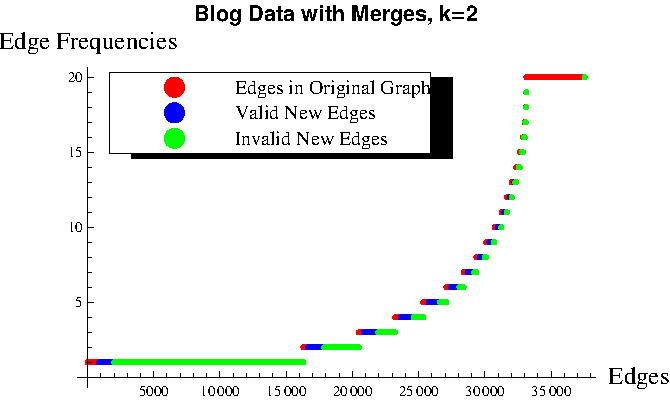
\includegraphics[width=1\linewidth]{s40_k_2_merges.pdf}
	\label{fig:Merging, k=2}
\end{subfigure}%
\begin{subfigure}{0.5\textwidth}
	\centering
	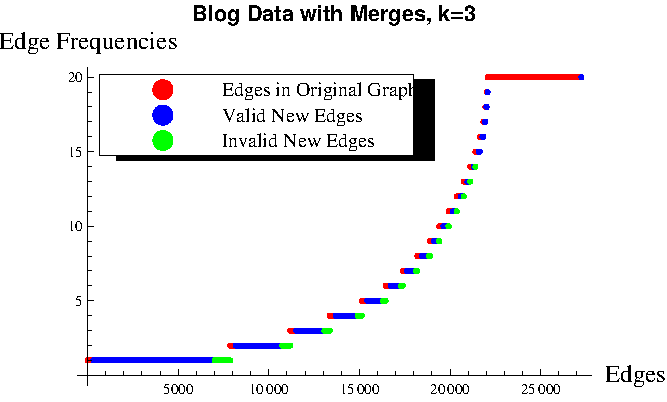
\includegraphics[width=1\linewidth]{s40_k_3_merges.pdf}
	\label{fig:Merging, k=3}
\end{subfigure}%
\caption{The results from the label-swapping algorithm when run 20 times on the blog data when k equals 2 and 3. Adjacency groups differing by 5 or less were merged. }
\end{figure}


%Edge Adding
\section{Edge Adding Algorithm}


\begin{figure}[htb]
	\begin{algorithmic}
		\renewcommand{\algorithmicrequire}{\textbf{Input:}}
		\renewcommand{\algorithmicensure}{\textbf{Output:}}
		\Require {Integer $k$, k-neighborhood graph $G=(V,E)$}
		\Ensure {Graph $G'=(V,E')$}
		\State {$wList=E$}
		\While {$wList \neq \emptyset$}
			\State {select and remove some $(u,v) \in wList$}
			\State {perform a BFS of length $k$ from $u \in V$}
			\If {BFS reaches $x \in V$ such that $x \not \in N_k(u)$}
				\State {skip}
			\EndIf
			\State {perform a BFS of length $k$ from $v \in V$}
			\If {BFS reaches $x \in V$ such that $x \not \in N_k(v)$}
				\State {skip}
			\EndIf
			\State {add $(u,v)$ to $E'$}
		\EndWhile
		\Return {$G'$}
	\end{algorithmic}
	\caption{Pseudocode for the Edge-Adding Algorithm}
	\caption{An example of the edge-adding algorithm. a) The 3-neighborhood graph for a given input. Each edge in this graph is added to the potential-edge list at the start of the algorithm. b) The solid lines represent edges that will be in the graph the algorithm returns (edge (B,D) was the last edge added). The dotted lines are remaining edges in the potential-edge list. After (B,D) was added, there became a 2-path between A and D. Since E is not adjacent to A in the 3-neighborhood graph, the edge (D,E) was removed from the potential-edge list.}
	\label{fig:edge-adding}
\end{figure}


\indent The edge-adding algorithm, as shown in figure \ref{edge-add}, is a greedy algorithm which find a graph $G = (V,E)$ that approximately satify a given k-neighborhood graph, $G_k = (V, E')$. The algorithm works to find a graph whose k-neighborhood is at least a subgraph of $G_k$. It begins by adding the edges of $G_k$ into a working list. We know any satisfying graph must be a subgraph of $G_k$, as every edge of a graph must be included in the k-neighborhood of that graph. Therefore, we want to find a subset of our working list that satisfies $G_k$. This algorithm works by iteratively adding edges from the working list to the new graph.  At each iteration, a random edge $(u,v)$ is selected and removed from the working list. A breadth-first search of length $k$ is run from both $u$ and $v$ in the current graph, $G$. If the search (say, from $u$) reaches a node that is not adjacent to $u$ in $G_k$, then we know adding $(u,v)$ to $G$ would invalidate the graph and the edge is discarded. If no such node is found, then $(u,v)$ is added to $G$. This process continues until the working list is empty. This algorithm runs in $O(|E|*d^k)$ time, where $d$ is the maximum node density. As social networking graphs are typically sparse, this algorithm runs in near-linear time.


%Adversary Simulation
\section{Adversary Simulation}

\noindent This section presents a simulated contest between a social networking website publishing neighborhoods and an adversary looking to determine existing edges from these neighborhoods. The website, knowing the original social network, uses the label-swapping algorithm multiple times and tracks the frequency each edge appears (edges that never occur in an output of label-swapping are ignored). For some $\epsilon,\delta \in [0,1]$, test the proportion of edges that occur with a frequency in $[0.5-\delta,0.5+\delta]$. If that proportion is less than $\epsilon$, increment $k$ and repeat the process. If $k$ reaches some set maximum (say 6), stop the process: k has become too large for the k-neighborhoods to hold any meaningful information. If the proportion is greater than $\epsilon$, set $k' = k$.  Figure \ref{k_vals} shows the determined k' values for various $\mu$ values. We belive that $k'$ is the minimum $k$ value to sufficiently disguise the given graph.

\indent To test this theory, we pass the k'-neighborhood of $G$ to the edge-adding algorithm and attempt to reconstruct $G$. The sucess of this attempt is measured by the proportion of edges the algorithm yields that are in $G$.

\begin{figure}[H]
  \label{k_vals}
  \centering
  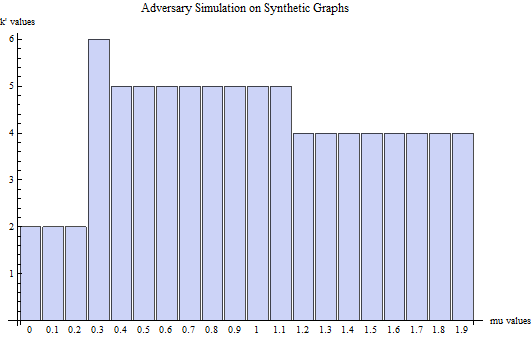
\includegraphics[scale=0.8]{k'_values.png}
  \caption{Returned k' values for synthetic graphs of different mu values.}
  \label{fig:k'_values}
\end{figure}

%Tests and Results
\subsection{Tests and Results}

\begin{figure}[ht]
  \centering
  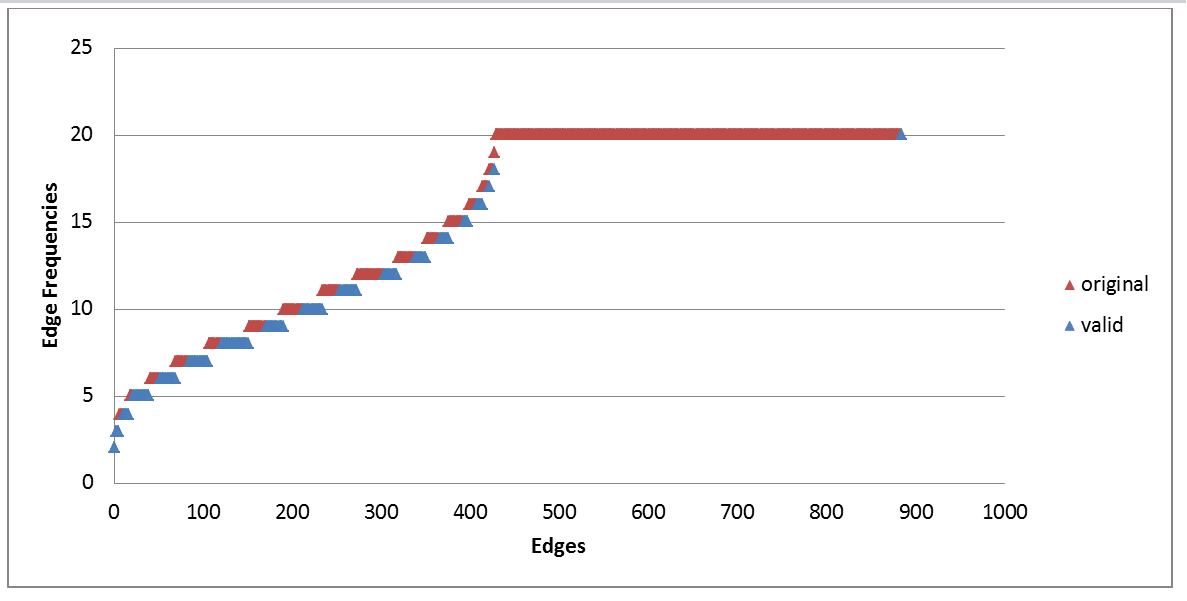
\includegraphics[scale=0.4 ]{mu=0_1 k=2 label.png}
  \caption{The results from the label-swapping algorithm when run 20 times on graphs whose mu value is 0.1 with k=2.}
  \label{fig:k=2 label-swap}
\end{figure}

\begin{figure}[ht]
  \centering
  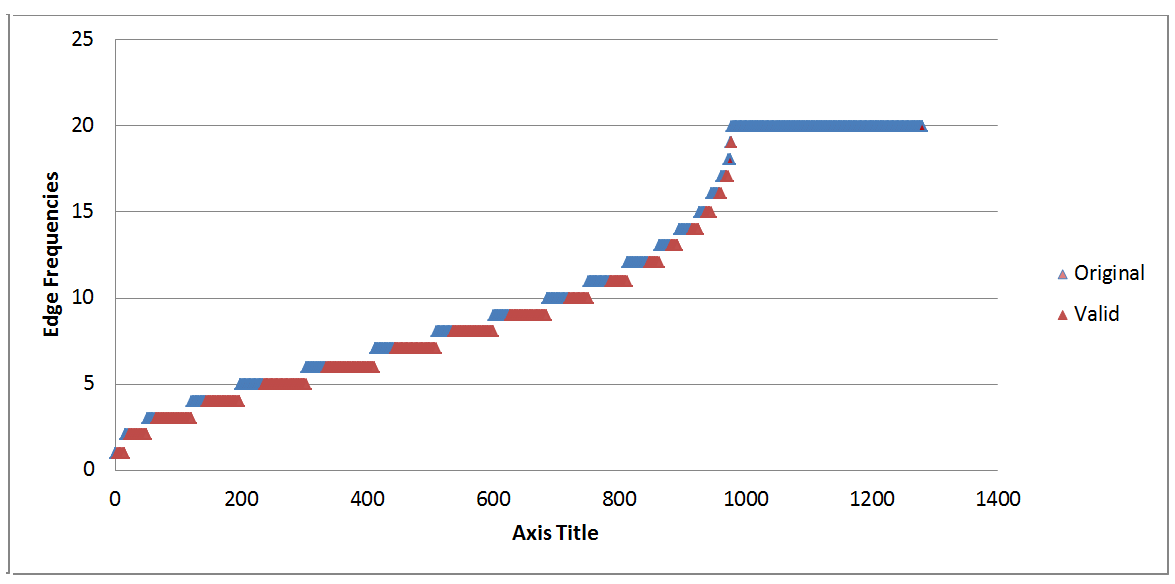
\includegraphics[scale=0.4 ]{mu=0_1 k=5 label.png}
  \caption{The results from the label-swapping algorithm when run 20 times on graphs whose mu value is 0.1 with a k=5 .}
  \label{fig:k=5 label-swap}
\end{figure}





\end{document}




